\vspace{-10pt}
\section{Experiments}\label{sect:experiments}
\vspace{-2pt}
In this section, we
conduct empirical evaluation of the proposed averaging protocol and its corresponding optimization algorithm. 
First, we check the theoretical properties of Moshpit All-Reduce in a controlled setup (Section~\ref{sect:experiments_averaging}). Then, we compare Moshpit SGD with other distributed methods on practical tasks of image classification and masked language model pretraining (Sections~\ref{sect:experiments_vision} and~\ref{sect:experiments_nlp}).

\vspace{-4pt}
\subsection{Decentralized averaging}
\label{sect:experiments_averaging}
In this series of experiments, we aim to empirically verify the convergence and fault tolerance properties proven in Section~\ref{sect:method_convergence}.
To measure this in a controlled setting, we create peers with parameters that are scalar values drawn from the standard Gaussian distribution. We study the convergence of different distributed methods with respect to the number of workers $N$ and their individual failure rate for a single iteration of averaging $p$  (failed peers return in the next round). 

We compare Moshpit Averaging with the following algorithms from prior work: All-Reduce (with restarts in case of node failures), Gossip, PushSum (equivalent to the method described in~\cite{sgpush}). Also, we provide the results of averaging in random groups as a simpler version of our approach. However, the implementation of group averaging maintains approximately the same group size across all iterations: this property might be hard to achieve in a decentralized setting, and as a result, the estimate of this method's performance should be considered highly optimistic.

We report the average squared difference between the worker parameters and the actual average of all values; the results are averaged across 100 restarts from different random initializations.
We compare the convergence for 512--1024 peers and consider failure probabilities ranging from 0 to 0.01. For Moshpit Averaging and random group averaging, we use groups of size 32, which corresponds to $M=32$ and $d=2$ for Algorithm~\ref{alg:moshpit}.

\vspace{-4pt}
\begin{figure}[h]
\noindent
\centering
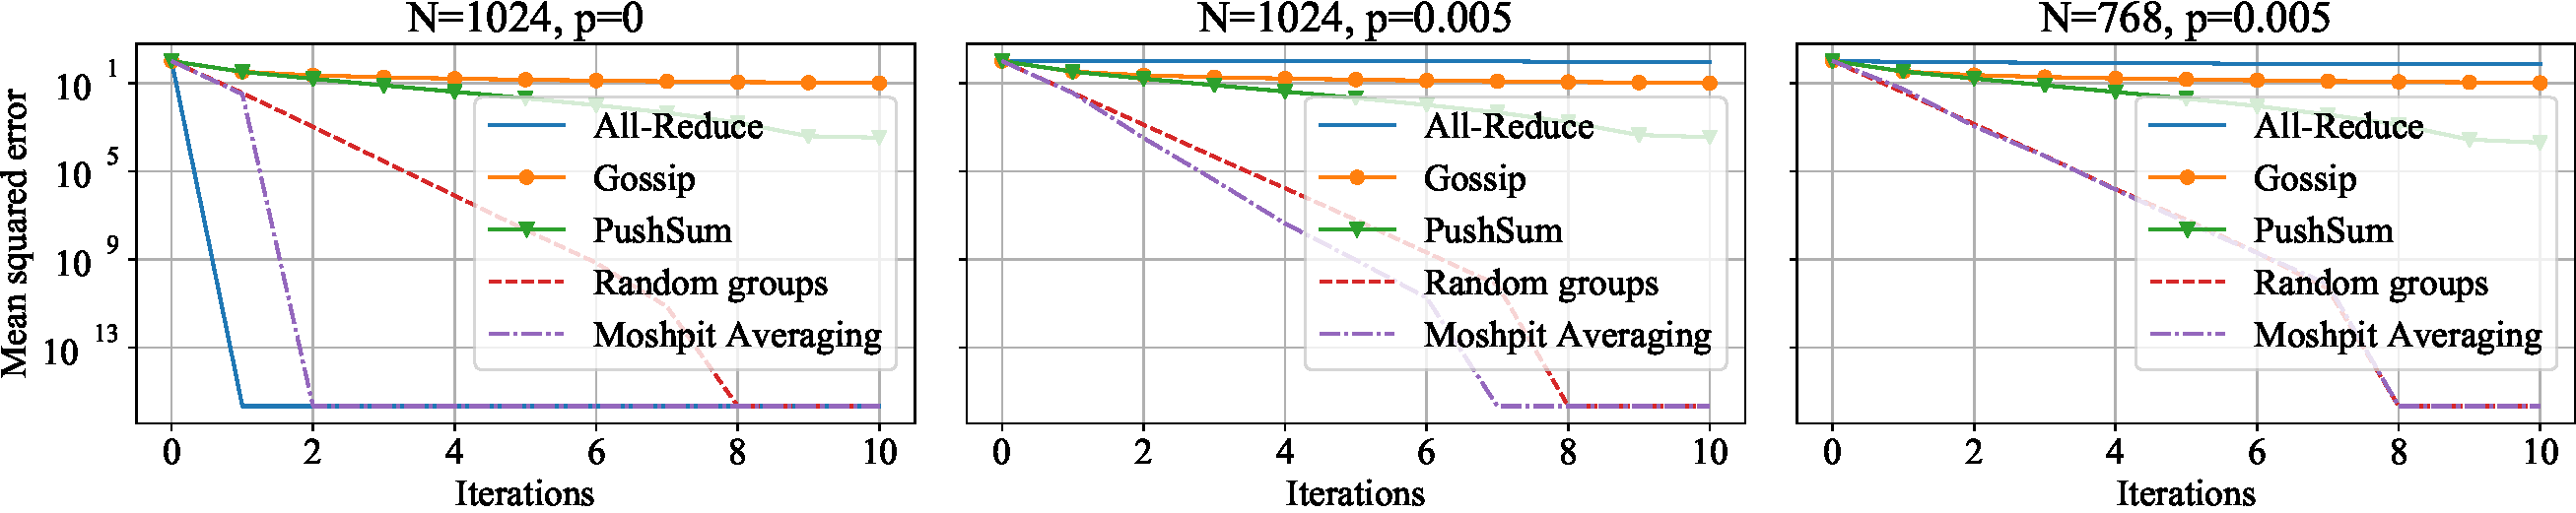
\includegraphics[width=\textwidth]{resources/averaging.pdf}
\caption{Convergence of averaging algorithms in different configurations.}
\label{fig:averaging}
\end{figure}
\vspace{-8pt}

Figure~\ref{fig:averaging} displays the results of experiments for several combinations of $N$ and $p$; the complete results with additional grid configurations are available in Appendix~\ref{sect:extra_averaging}. We make several key observations: 
\begin{enumerate}[leftmargin=*]
    \vspace{-2pt}\item When the failure rate of each peer is zero, standard All-Reduce predictably computes the average faster than all other methods. However, as soon as $p$ reaches a value of at least 0.005, the number of retries needed for the success becomes prohibitively high.
    \vspace{-2pt}\item Previous decentralized averaging methods, such as Gossip or PushSum, require significantly more iterations for convergence to the global average than Moshpit All-Reduce, likely due to the structure of their communication graphs.
    \vspace{-2pt}\item As discussed in Section~\ref{sect:method_algorithm}, when the total number of peers is equal to the grid capacity and there are no failures, Moshpit All-Reduce matches the result of regular All-Reduce with the number of steps equal to the number of grid dimensions (2 in this case).
    \vspace{-2pt}\item Averaging in random groups can perform comparably to Moshpit Averaging when the number of peers is less than half of the grid capacity. The reason for this behavior is that when the workers do not fully occupy the grid, the group sizes are no longer guaranteed to be equal across groups and across iterations. In the worst case, there can be groups of only one peer for certain grid coordinates, which may significantly affect the convergence. However, as the grid utilization grows, Moshpit Averaging starts to outperform random group averaging. Moreover, even if we use 512 peers, arranging them in a proper 8x8x8 grid leads to faster convergence.
\end{enumerate}

\pagebreak[4]


\subsection{ImageNet training}\label{sect:experiments_vision}
Here, we evaluate the performance of Moshpit SGD in distributed training. More specifically, we train ResNet-50~\cite{resnet} on the ILSVRC~\cite{imagenet_cvpr09} dataset, following the training protocol of~\cite{goyal2017accurate}. Trainers use SGD with Nesterov momentum with a batch size of 256 and 32-bit precision regardless of the GPU type\footnote{For GPUs that cannot fit this into memory, we accumulate gradients over 2 batches of 128 examples.}. We evaluate the following training strategies:
\begin{itemize}[leftmargin=*]\vspace{-2px}
    \item \textbf{All-Reduce SGD (AR-SGD)} --- traditional distributed training with all-reduce gradient averaging;
    \item \textbf{Asynchronous Decentralized Parallel SGD (AD-PSGD)} --- parallel SGD that runs gossip communication in a cycle: each worker averages parameters with 2 neighbors~\cite{ad_psgd}. Communication rounds are overlapped with computation;
    \item \textbf{Stochastic Gradient Push (SGP)} --- a more advanced algorithm with an exponential communication graph and push-based communication~\cite{sgpush};
    \item \textbf{Moshpit SGD} --- similar to \textbf{SGP}, but with 1 round of Moshpit Averaging instead of PushSum.
\end{itemize}\vspace{-2px}

We report top-1 validation accuracy as a function of training time in two experimental setups:
\begin{itemize}[leftmargin=*]\vspace{-4px}
    \item \textbf{Homogeneous}: 16 servers with a single Tesla V100-PCIe GPU, 6 CPU cores, and 64GB RAM.
    \item \textbf{Heterogeneous}: a total of 81 GPUs (V100, 1080Ti, and P40) across 64 servers and workstations.\footnote{We provide a detailed configuration in Appendix~\ref{sect:detailed_setup}.}
\end{itemize}\vspace{-4px}

All servers and workstations communicate over the network with 1Gb/s Ethernet (non-dedicated symmetric bandwidth). The machines are located in two data centers and one office within 300 km of one another. The communication latency is 1--6ms depending on the location. To simulate shared usage, at the beginning of each communication round we inject additional latency sampled from the exponential distribution~\cite{sukhov2016generating} with the mean of 100ms.

For Moshpit SGD, we use a two-dimensional ``grid'' with 4 and 8 groups for homogeneous and heterogeneous setups respectively. For AD-PSGD, we attempt to compensate for slow convergence by training for 60 more epochs without changing the learning rate schedule. Finally, we only report AR-SGD in the first setup, as it is unsuitable for heterogeneous hardware.%



The results in Figure~\ref{fig:all} (Left) demonstrate that the two most efficient strategies for our setting are Moshpit SGD and SGP. In the \textbf{homogeneous} setup, Moshpit is only slightly more efficient than SGP, likely due to higher efficiency of all-reduce. This advantage increases to over 30\% for the \textbf{heterogeneous} setup with 64 servers. In turn, AR-SGD demonstrates the best performance per iteration, but its training time is by far the longest due to network latency ($1.5{\times}$ of Moshpit SGD). Finally, AD-PSGD predictably shows the best throughput (time per epoch), but achieves lower accuracy even after training for 150 epochs. We report results for smaller setups in Appendix~\ref{sect:extra_classification}. %


\subsection{Masked Language Model training}
\label{sect:experiments_nlp}
Finally, we evaluate Moshpit All-Reduce training performance in the wild with preemptible cloud instances. For this experiment, we perform one of the most resource-demanding tasks in modern deep learning --- unsupervised pretraining of Transformers~\cite{bert,roberta,radford2019language,gpt3}.
We opt for the ALBERT model~\cite{albert} to make better use of communication-constrained devices. This model has fewer trainable parameters due to layer-wise weight sharing.

\begin{figure*}[t]
    \noindent
    \centering
    \vspace{-10pt}
    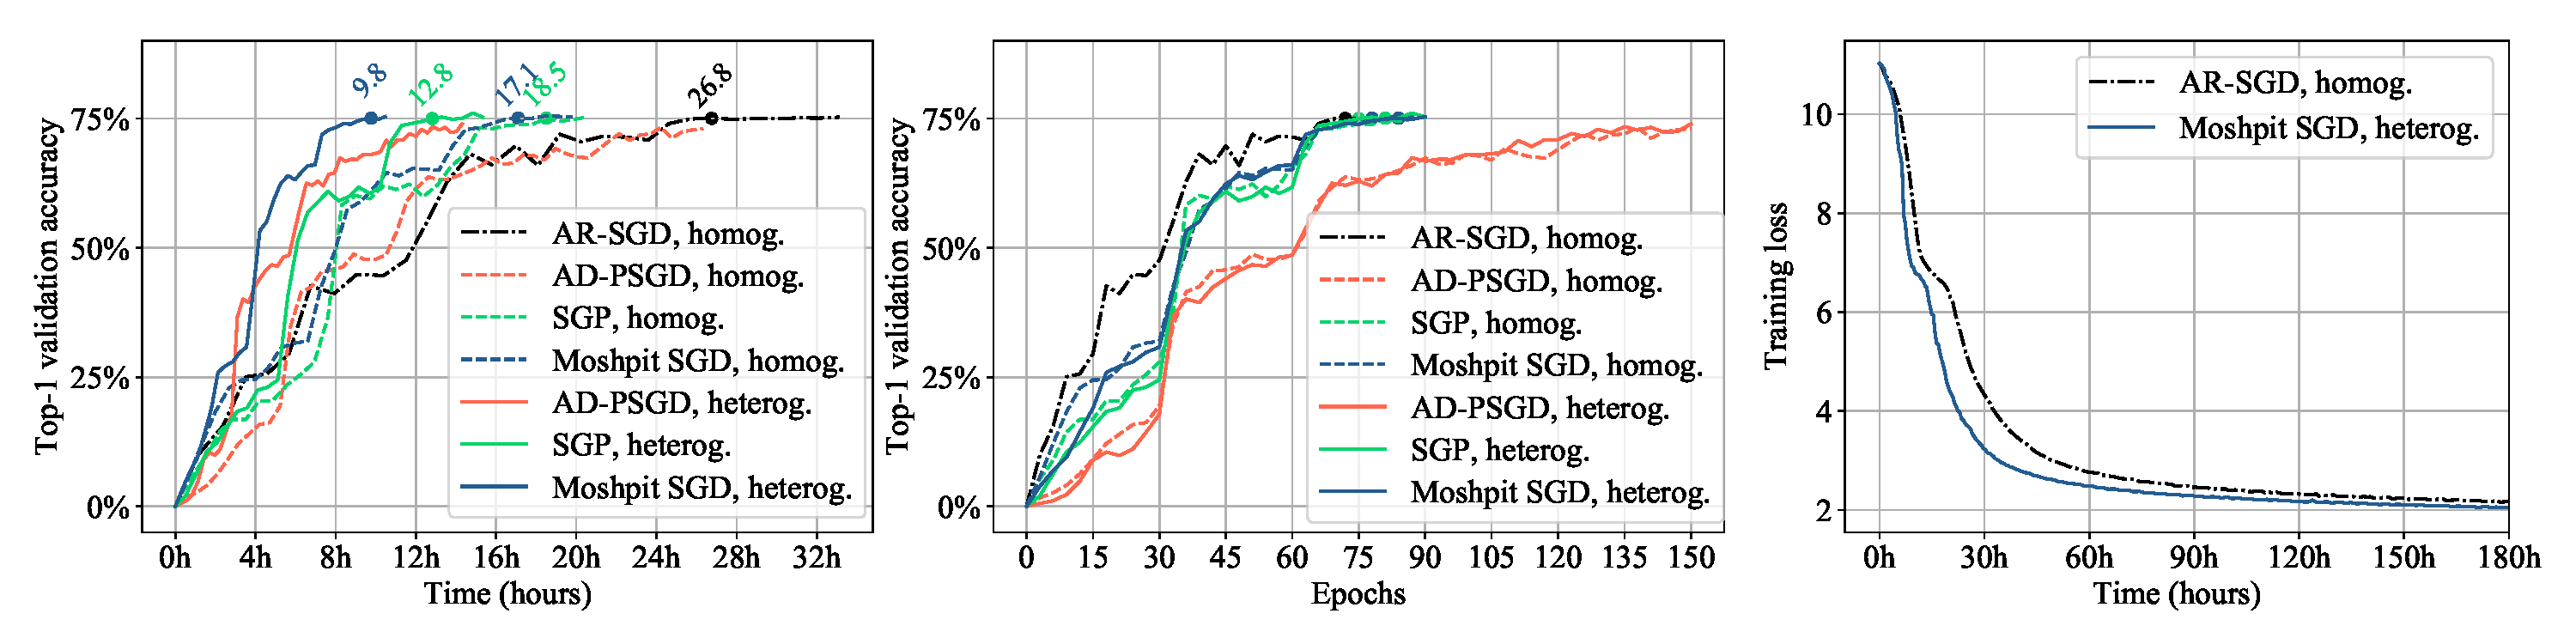
\includegraphics[width=\textwidth]{resources/albert_hours.pdf}
    \vspace{-16pt}
    \caption{\textbf{(Left, Middle)} ResNet-50 top-1 validation accuracy for ImageNet as a function of training time (left) and epochs (middle). \textbf{(Right)} Full training objective (MLM + SOP) of ALBERT-large on BookCorpus as a function of training time.}
    \label{fig:all}\vspace{-6pt}
\end{figure*}


Specifically, we train ALBERT-large (18M parameters) on the BookCorpus~\cite{bookcorpus} dataset, following the training setup from the original paper. We minimize the masked language modeling loss (MLM) along with the sentence order prediction loss (SOP) using the LAMB optimizer~\cite{You2020Large} with a global batch size of 4096 and sequence length 512. We measure convergence in terms of full training loss~\cite{lin2020multinode,fedus2021switch}. Similarly to Section~\ref{sect:experiments_vision}, we use two training setups:
\vspace{-4pt}\begin{itemize}[leftmargin=*]
    \item \textbf{Homogeneous:} a single cloud instance with $8$ Tesla V100-PCIe GPUs and 56 vCPUs;
    \item \textbf{Heterogeneous:} a total of 66 preemptible GPUs, 32 of which are cloud T4, and the remaining 34 are various devices rented on a public marketplace.
\end{itemize}\vspace{-4pt}

Despite the fact that the latter setup has almost $3{\times}$ more raw compute\footnote{Based on official performance benchmarks~\cite{nvidia_perf}.}, its hourly rent costs less than the homogeneous setup due to relying on preemptible instances\footnote{Please refer to Appendix~\ref{sect:detailed_setup} for full experimental setups.}. This instance type is much cheaper than regular cloud instances, but it can be interrupted at any time. As a side-effect, the participants in \textbf{heterogeneous} setup are also spread across 3 continents with uneven network bandwidth, ranging from 100Mb/s to 1500Mb/s per worker. These limitations make it impractical to deploy conventional all-reduce protocols. By contrast, the fully decentralized nature of Moshpit SGD allows it to operate on unreliable nodes.

In this setup, the participants accumulate gradients over multiple local batches and use DHT to track the global batch size. Once the swarm collectively accumulates gradients over 4096 training samples, it runs 2 rounds of Moshpit All-Reduce with $M{=}8$ and $d{=}2$. Unfortunately, training with simple parameter averaging does not converge, likely due to diverging LAMB statistics. To mitigate this issue, workers recover ``pseudo-gradients''~\cite{reddi2021adaptive,chen2020toward} after averaging to update the optimizer statistics.




Figure~\ref{fig:all} (right) demonstrates that Moshpit SGD with a fully preemptible fleet of machines trains 1.5 times faster than the traditional data-parallel setup.
The final loss achieved by two training strategies is the same within the margin of error.
A closer investigation reveals that this speedup is entirely explained by the reduced iteration time.
An interesting observation is that the iteration time of Moshpit SGD varies between {10--22} seconds, while AR-SGD consistently spends {25}s per step. This can be explained by natural variation in the preemptible fleet size: there were 30--66 active participants depending on the resource availability.
